% !TEX spellcheck = en_US

\documentclass[10pt,journal,compsoc]{IEEEtran}




%: ~~~~~~~~~~~~~~~~~~~~~~~~~~~~~~~~~~~~~~~ V HB Packages v2021-04-01
	\usepackage[utf8]{inputenc} 
	\usepackage[iso]{datetime}
	\newcommand{\hbTimeStamp}{{\color{red}--Draft-- v\today/\currenttime}} % version
	\usepackage{amssymb}
	\usepackage{enumerate}
	
	\usepackage[a4paper]{geometry}
	
	\usepackage{xcolor}
	% black, blue, brown, cyan, darkgray, gray, green, lightgray, lime, 
	% magenta, olive, orange, pink, purple, red, teal, violet, white, yellow
		\definecolor{darkred}{rgb}{0.8,0.1,0.1}
		\definecolor{darkgreen}{rgb}{0,0.5,0}
		\definecolor{darkblue}{rgb}{0,0,0.5}
		\colorlet{RED}{red}
	
	\usepackage[colorlinks=true,linkcolor=red,urlcolor=blue,citecolor=red]%
		{hyperref}
	\usepackage{graphicx,epstopdf}
	% \graphicspath{{fig}}
	\graphicspath{{../common/figures/}}
	% \DeclareGraphicsExtensions{.pdf,.jpeg,.png,.eps}
	% \DeclareGraphicsRule{.tif}{png}{.png}%
	%	{`convert #1 `dirname #1`/`basename #1 .tif`.png}
%	\usepackage{subfigure}
%	\usepackage{subfig}
	\usepackage{subcaption}
% ~~~~~~~~~~~~~~~~~~~~~~~~~~~~~~~~~~~~~~~ A




%: ~~~~~~~~~~~~~~~~~~~~~~~~~~~~~~~~~~~~~~~ V HB Declarations v2021-04-01
	\newcommand{\reffig}[1]{Fig.~\ref{#1}}
	\newcommand{\refeq}[1]{Eq.~\ref{#1}}
	\newcommand{\reftbl}[1]{Table~\ref{#1}}
	\newcommand{\refsec}[1]{Sec.~\ref{#1}}
	\newcommand{\refcite}[1]{Ref~\cite{#1}}
	\newcommand{\refalg}[1]{Algorithm~\ref{#1}}
	\newcommand{\reflst}[1]{List.~\ref{#1}}  % code listing
	%
	\newcommand{\refthm}[1]{Theorem~\ref{#1}}
	\newcommand{\refthmA}[2]{\refthm{#1}(\ref{#2}}
	\newcommand{\reflem}[1]{Lemma~\ref{#1}}
	\newcommand{\refdef}[1]{Definition~\ref{#1}}
	\newcommand{\refexmp}[1]{Example~\ref{#1}}
	%
	\newcommand{\hQuote}[1]{{\small \textsf{``#1''}}}
	\newcommand{\hCode}[1]{\texttt{#1}}
	\newcommand{\hIdea}[1]{{\color{olive}{\scriptsize [{#1}]}}}
	\newcommand{\hFootnote}[2]{\footnote{{\color{red} @#1 : }#2}}
% ~~~~~~~~~~~~~~~~~~~~~~~~~~~~~~~~~~~~~~~ A




%: ~~~~~~~~~~~~~~~~~~~~~~~~~~~~~~~~~~~~~~~ V HB Math v2021-04-01
	\usepackage{amsmath, amssymb,amsfonts,amsthm}
	%
	\theoremstyle{plain}
	\newtheorem{thm}{Theorem}[section]
	\newtheorem{lem}[thm]{Lemma}
	\newtheorem{prop}[thm]{Proposition}
	\newtheorem*{cor}{Corollary}
	\theoremstyle{definition}
	\newtheorem{defn}{Definition}[section]
	\newtheorem{conj}{Conjecture}[section]
	\newtheorem{exmp}{Example}[section]
	\theoremstyle{remark}
	\newtheorem*{rem}{Remark}
	\newtheorem*{note}{Note}
	%
	\newcommand{\hDefined}[1]{\textcolor{darkred}{\textit{#1}}}	
	\newcommand{\hVec}[1]{\mathbf{#1}}	 
	\newcommand{\hAbs}[1]{\ensuremath{\left \lvert \, #1 \, \right \rvert} } % |x|
	\newcommand{\hMat}[1]{\mathbf{#1}}
	\newcommand{\hArgmin}[2]{\underset{#1}{\operatorname{arg \, min}}\;#2}
	\newcommand{\hArgmax}[2]{\underset{#1}{\operatorname{arg \, max}}\;#2}
% ~~~~~~~~~~~~~~~~~~~~~~~~~~~~~~~~~~~~~~~ A




\hyphenation{
	op-tical net-works semi-conduc-tor
}





% ~~~~~~~~~~~~~~~~~~~~~~~~~~~~~~~~~~~~~~~ V
\begin{document}

\title{
	Title of the paper
}

\author{
	YourName~Lastname,
	Haluk~O.~Bingol
	\IEEEcompsocitemizethanks{
		\IEEEcompsocthanksitem Y. Lastname and H. O. Bingol  are with Bogazici University.
	}%
%	\thanks{
%		Manuscript received April 19, 2005; 
%		revised August 26, 2015.
%	}%
}

\markboth{
	\hbTimeStamp
}%
{
	\hbTimeStamp
}

\IEEEtitleabstractindextext{%
	\begin{abstract}
		The abstract goes here.
	\end{abstract}
	
	\begin{IEEEkeywords}
		KeywordA, keywordB.
	\end{IEEEkeywords}
}

\maketitle
% ~~~~~~~~~~~~~~~~~~~~~~~~~~~~~~~~~~~~~~~ A




% ~~~~~~~~~~~~~~~~~~~~~~~~~~~~~~~~~~~~~~
\section{Introduction}

Aaa.




% ~~~~~~~~~~~~~~~~~~~~~~~~~~~~~~~~~~~~~~
\subsection{A few reminders}

It would be better if you clone git repository 
\href
	{https://github.com/halukbingol/LaTeX-Templates}
	{https://github.com/halukbingol/LaTeX-Templates}.
Frequently pull to get updates.
	
Please compile and read 
\href
	{https://github.com/halukbingol/LaTeX-Templates/tree/master/bingol-MyLaTeXBestPractices}
	{MyLaTeXBestPractices} 
in this repo first.


% +++++++++++++++++++++++++++++++++++++++ V
%: -Fig.
\begin{figure}[htbp]
\begin{center}
	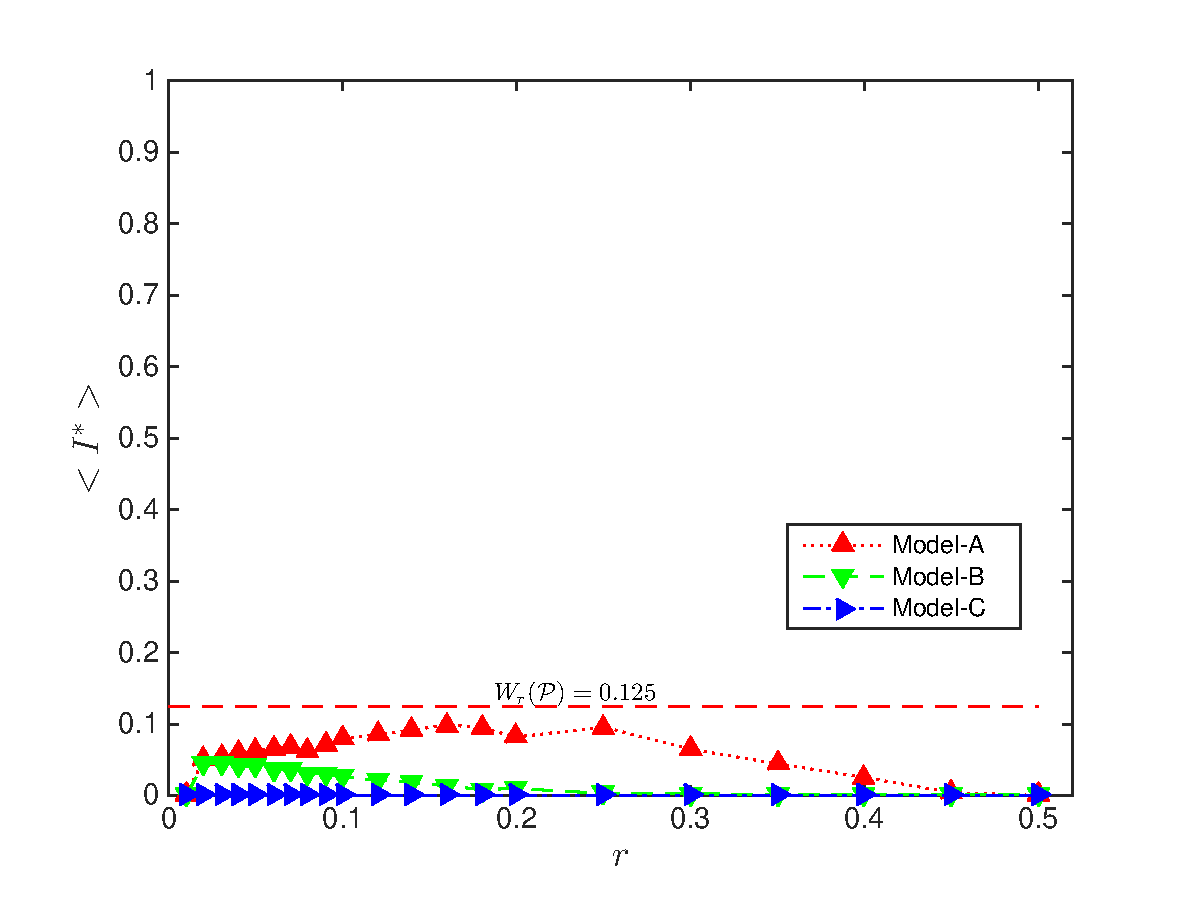
\includegraphics[width=\columnwidth]
		{Fig-FigureA}
	\caption{Household layer.}
	\label{fig:figureA}
\end{center}
\end{figure}
% +++++++++++++++++++++++++++++++++++++++ A




% ~~~~~~~~~~~~~~~~~~~~~~~~~~~~~~~~~~~~~~
\section{Related work}

Aaa.




% ~~~~~~~~~~~~~~~~~~~~~~~~~~~~~~~~~~~~~~
\section{Our model/method}

Aaa
\begin{align}
	x = y
	\label{eq:bbb}
\end{align}
bbb.




% ~~~~~~~~~~~~~~~~~~~~~~~~~~~~~~~~~~~~~~
\section{Finding/Discussion}

Aaa.





% ~~~~~~~~~~~~~~~~~~~~~~~~~~~~~~~~~~~~~~
\section{Conclusion}

Aaa.




\section*{Acknowledgment}

The authors would like to thank Aaaa.
%
This work is partially supported by 
the Turkish Directorate of Strategy and Budget
under the TAM Project number 2007K12-873.


\bibliographystyle{IEEEtran}
\bibliography{bingol-template-paper}


\end{document}


